\documentclass[journal, a4paper]{IEEEtran}

\usepackage{cite}
\usepackage{amsmath}
\usepackage{amssymb}
\usepackage{graphicx}
\usepackage{url}
\usepackage[usenames, dvipsnames]{color}

\begin{document}

\title{Scaling of Electrode-Electrolyte Interface Model Parameters In Phosphate Buffered Saline}

\author{Mark~H.~Jones and Jonathan~Scott,~\IEEEmembership{Senior Member,~IEEE}

\thanks{Mark~H.~Jones is with the School of Electronic Engineering, University of Waikato, New Zealand, e-mail: markjones112358@gmail.com.}%

\thanks{Jonathan Scott is with the School of Electronic Engineering, University of Waikato, New Zealand.}

}

\markboth{Transactions on Biomedical Circuits and Systems}
{Jones \MakeLowercase{\textit{et al.}}: Scaling of Electrode-Electrolyte Interface Model Parameters in Phosphate Buffered Saline\...}
\maketitle

\begin{abstract}
We report how the impedance presented by a platinum electrode scales with the concentration of phosphate buffered saline (PBS).
We find that the constant phase element of the model scales with approximately the log of concentration, whereas the resistivity is inversely proportional.
Using a novel DC measurement technique we show that the Faradaic response of a platinum electrode, and thus the safe exposure limit, does not scale with concentration below 900\thinspace mV overpotential across a pair of electrodes.
We compare objective measurements made in saline to those made in the spinal cavity of live sheep. We comment upon the appropriateness of using PBS as a substitute for living sheep.
\end{abstract}

\begin{IEEEkeywords}
    Electrical stimulation, Bioelectric phenomena, Biophysics, Bioimpedance, Biomedical electrodes, Biomedical measurements, Implantable biomedical devices
\end{IEEEkeywords}

\section{Introduction}
\IEEEPARstart{T}{here} is considerable interest in the electrical modelling of electrodes. \cite{Cogan2008,Troy2006}
In \cite{Franks2005} a linearised model was presented, and in \cite{ScottSingle2013} a non-linear model
suitable for use with the SPICE circuit simulator was presented. The SPICE model usefully characterises an electrode in a given electrolyte with a small number of parameters.
One major reason for the interest in the electrical impedance of electrodes concerns the design of electronics intended for integration into pacemakers, cochlear implants, spinal cord stimulators, etc. The design of successful circuits depends upon a good understanding of external load impedance, while maximisation of battery life is linked to the use of electrodes whose impedance is well understood.
Having a compact model of an electrode in the appropriate electrolyte allows circuit designers to simulate their designs with valid loads. Knowing the effect upon the model of changes in the electrode or electrolyte would allow designers to anticipate circumstances that will affect the load seen by their circuits. Another appeal of a compact model stems from the fact that electrode characteristics are succinctly and objectively represented by the model parameters. These enable direct comparison of different electrodes, or the change in electrode properties over time. For example, in \cite{Kane13} changes in chronically-implanted electrodes are observed but there is no standard quantitative way of presenting the changes. Similarly, while there is a good understanding of what represents safe exposure, a compact model with parameters permits the prediction of the safety of any given stimulus regime.~\cite{Merrill05}

Electrodes in the laboratory are typically tested in a saline solution selected to mimic the circumstances in which they will operate when implanted.
{
    \color{blue}
    % Item 20
A solution of Phosphate Buffered Saline (PBS) diluted to one-tenth concentration (0.1X) is common in the case of Spinal Cord Stimulators (SCS), while full concentration (1.0X) PBS is considered more representative of the situation in blood.
}
In this manuscript we report how the parameters of a non-linear model change as the concentration of saline is varied. {\color{blue} We refine a series of measurements compatible with commercially available medical electrodes in physiological saline that allow us to describe the impedance with minimal parameters.} We place these parameters in context with a biological measurement made in the spinal cavity of a live sheep.

The electrode used in this work is a commercial linear array of eight platinum electrodes intended for SCS implantation called an ``Octrode''.~\cite{StJudeOctrode} A picture of an Octrode is presented in figure~\ref{fig:octrode}.
The electrical interface model of \cite{Franks2005} and \cite{ScottSingle2013} has two parts, a displacement branch and a Faradaic branch. {\color{blue} While Scott and Single \cite{ScottSingle2013} incorporate a memristor into their model, it has been omitted here for simplicity. Its contribution is limited to situations where diffusion limited Faradaic reactions come into play, a situation that stimulator implants are designed to avoid.}

{
    \color{blue}
It has been suggested that the primary coupling mechanism between platinum electrodes and physiological saline is the reversible evolution of gas, probably oxygen, at the platinum surface, which dissolves without bubble formation.\cite{Greatbatch1969} Understanding exact mechanism of displacement or Faradaic charge transfer at the electrode surface is beyond the scope of this work, instead we wish to characterise the electrode/electrolyte system in terms of parameters that may be fed into an electrical model. 
}

\begin{figure}
    \begin{center}
    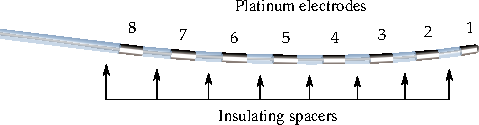
\includegraphics{graphics/StJudeOctrodeDiagram}
    \end{center}
    \caption{St. Jude Medical Octrode lead comprised of eight coaxial cylindrical platinum electrodes (1mm in diameter, 3mm long) separated by 4mm insulating spacers.}
    \label{fig:octrode}
\end{figure}

\begin{figure}
    \begin{center}
        
\includegraphics[width=230pt]{graphics/interfaceSchematic_noMemristive}
    \end{center}
    \caption{Electrical schematic of the electrode-interface impedance model used in this work. $D_{a}$ and $D_{b}$ represent diodes; $CPE$ and $R_{s}$ represent the constant phase element and series resistance respectively.}
    \label{fig:schematic}
\end{figure}

\section{Resistive Network}
Six solutions ranging from 1.0X to 0.025X the concentration of a stock PBS solution have been examined.
The ingredients of that stock solution are given in table~\ref{tab:PBSrecipe}.
{
    \color{blue}
    % Item 11
    The pH level of the stock was measured, using a calibrated EDT Instruments BA-350 pH meter, to have a pH of 7.4. No pH adjustments were made to the derived solutions.
}
\begin{table}
    \begin{center}
        \begin{tabular}{|r|l|}
            \hline
            $NaCl$ & $8.0\thinspace g$ \\ \hline
            $KCl$ & $0.2\thinspace g$ \\ \hline
            $Na_{2}HPO_{4}$ & $1.44\thinspace g$ \\ \hline
            $KH_{2}PO_{4}$ & $0.24\thinspace g$ \\ \hline
            Distilled Water & $1.0$\thinspace L \\ \hline
        \end{tabular}
    \end{center}
    \caption{PBS stock solution ingredients}
    \label{tab:PBSrecipe}
\end{table}

The electrical impedance between two electrodes in an electrolyte arises from two interface impedances in series with the resistance due to the bulk of the electrolyte itself. To quantify the impedance presented by a single interface we first need to understand the inter-electrode resistances presented by the electrolyte bulk. As there are always two interface impedances between any two electrodes, inter-electrode resistances cannot be measured in isolation.

In \cite{ScottSingle2013}, a series of transresistance measurements were used in conjunction with a physical description of the electrode geometry to build up a representative network of resistors. The network in that paper was defined using five parameters: $R_{eri}$, $R_{lri}$, $R_{li}$, mesh depth, and edge depth. Readers are advised to read that paper to understand the interpretation of these model parameters. Repeating that work, a resistor network that connects each of the eight electrodes is constructed, mimicking the resistances due to the solution bulk.
{
    \color{blue}
The mesh depth and padding values of five columns and three rows, respectively, has been taken directly from \cite{ScottSingle2013}.
A numerical fit was made to the two independent scaling parameters $R_{eri}$ and $R_{li}$
\footnote{The values of $R_{eri}$ and $R_{sri}$ are defined by the lengths of the electrode and inter-electrode spacers respectively as described in \cite{ScottSingle2013}. The two parameters are proportional to each other by the ratio of their lengths. Hence, we define $R_{sri}$ to be 3/4 that of $R_{eri}$ making it a dependant parameter.}.
}
The resulting fit and parameter values are presented in figure~\ref{fig:transresistance} and table~\ref{tab:RESparams} respectively. 
{
    \color{blue}
    % Item 11
Measurements of the inter-electrode impedance were made using a Tektronix TPS2014 DSO with four fully isolated and floating channels; an Agilent 33220A Function Generator; and a desktop PC controlling the instruments via Python 2.7.
}

\begin{figure}
    \begin{center}
        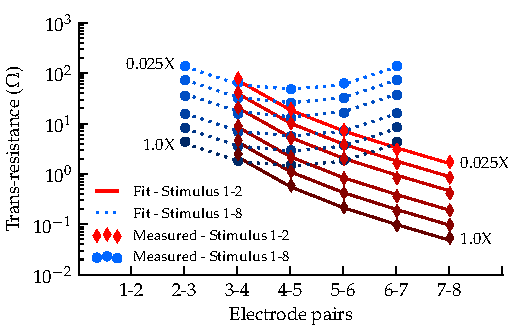
\includegraphics{graphics/pbs_transimpedance_IEEE}
    \end{center}
    \caption{Transresistance measurements (markers) used to generate the resistor mesh and the corresponding fit (lines). Red diamonds indicate results where a stimulus is placed across electrodes 1 and 2. Blue circles represent measurements where the stimulus is placed across electrodes 1 and 8. Each trace represents one of six concentrations of PBS, increasing in transresistance magnitude monotonically from 1.0X to 0.025X.}
    \label{fig:transresistance}
\end{figure}

\begin{table}
    \begin{center}
        \begin{tabular}{|r|l|}
            \hline
            $R_{eri}$ & 0.407 / $\sigma$ \\ \hline
            $R_{sri}$ & $R_{eri}$ $3/4$ \\ \hline
            $R_{li}$ & 3.71 / $\sigma$ \\ \hline
            Depth & 5 layers \\ \hline
            Padding & 3 layers \\ \hline
        \end{tabular}
    \end{center}
    \caption{Resistor mesh parameters. $\sigma$ measured in units of $S/cm$}
    \label{tab:RESparams}
\end{table}


\section{Displacement Parameters}
{
    % Identifying reactions
    \color{blue}
Displacement currents are responsible for capacitive behaviour at interfacial boundaries.
They are brought about by the redistribution of charge in response to applied fields, i.e. a charged electrode will attract or repel $Cl^{-}$ from its surface and reorientate polar molecules in the surrounding solution. This capacitive behaviour may also be a result of electrode polarisation in the form of reversible Faradaic reactions at the surface of the electrode.
Such reactions involving water and platinum, as identified in \cite{Horch2004,Mohtashami2011}, include:
    \begin{eqnarray}
        Pt + H_{2}O &\Leftrightarrow& PtO + 2 H^{+} + 2 e^{-}\\
        PtO + H_{2}O &\Leftrightarrow& PtO_{2} + 2 H^{+} + 2e^{-}\\
        Pt + H^{+} & \Leftrightarrow & Pt-H\\
        Pt + H_{2}O + e^{-} &\Leftrightarrow& Pt-H+OH^{-}
    \end{eqnarray}

This displacement mechanism is capable of transferring charge between electrical and biological systems without damaging electrodes or tissue. \cite{Horch2004}
This behaviour is modelled by way of a Constant Phase Element (CPE); also known as a fractional capacitor.
}
For simulation purposes this element is realised as an array of R-C branches.~\cite{ScottSingle2013,Morrison59,Elwakil10} We measured displacement currents by sweeping the frequency of a sinusoidal stimulus across electrodes 2 and 7 of the Octrode while measuring the voltage between electrodes 2 and 3. 
The numbering pattern used to identify each of the electrodes on the Octrode is shown in figure~\ref{fig:octrode}.
Measurements made using this configuration allow for the quantification of a single interface impedance in series with the resistance presented by the bulk solution.
{
    \color{blue}
Current density during measurements peaked at $11.5\thinspace A/m^{2}$ at 10\thinspace kHz in 1.0X PBS and fell as low as $0.0141\thinspace A/m^{2}$ at 50\thinspace mHz in 0.025X PBS. The stimulus waveform was set at 300\thinspace mV (peak) at each measurement point. The measurement insturments used are the same as those used to measure the inter-electrode resistance.
}
{
    \color{blue)
    % Item 6
    Figure~\ref{fig:CPE_Magnitude} shows the magnitude of the measured response of each of the six PBS concentrations accompanied by simulation results. Figure~\ref{fig:CPE_Phase} shows the phase response for the same measurements, again with the simulated response at each concentration. The simulated responses are generated using the optimised parameter values presented in Table~\ref{tab:CPEparams}. Those values were chosen as they give the closest match to the measured data. 
}
As shown in the interface model schematic (figure~\ref{fig:schematic}), the interface contains its own internal series resistance ($R_{S}$). The resistance seen in series with the CPE will therefore be the sum of both the resistance due to the bulk resistivity of the fluid and $R_{S}$, to which we will refer as $R_{S+bulk}$.
In figure~\ref{fig:CPE_Magnitude}, the slope and magnitude of the CPE are visible below 1\thinspace Hz whereas $R_{S+bulk}$  dominates above 1\thinspace kHz; it is clear that the two do not scale similarly.
As the impedance of the CPE and $R_{S+bulk}$ are separable with frequency, these measurements can be used to determine the CPE parameters and $R_{S}$.

Figure~\ref{fig:CPE_Scaling} shows measured data and the corresponding fits for both the CPE magnitude at 0.05\thinspace Hz and $R_{S+bulk}$. The resulting model parameters $m$, $k$, and $|Z|\thinspace @\thinspace 1Hz$ are shown in table~\ref{tab:CPEparams}. Here we express the CPE offset parameter as $|Z|\thinspace @ \thinspace 1Hz$, but the fits used $|Z|\thinspace @ \thinspace 0.05Hz$, as data points at this frequency are outside the transitional zone where the impedance of the CPE and that of $R_{S+bulk}$ overlap.

From the results shown in figure~\ref{fig:CPE_Magnitude} we observe that the salinity of the electrolyte does not affect the slope of the CPE's impedance and the magnitude shifts relatively little. This suggests that the CPE does not rely on the added ions but they do have an effect, implying that its behaviour is a property of platinum and $H_{2}O$.

\begin{figure}
    \begin{center}
        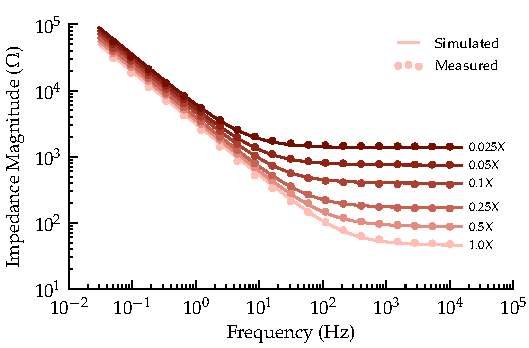
\includegraphics{graphics/displacement_impedanceVsFrequency_magnitude}
    \end{center}
    \caption{Magnitude of interfacial impedance between electrodes 2 and 7 against the frequency of a sine wave stimulus for six concentrations of PBS. The slope of the CPE is visible the left, whereas the resistance due to the solution bulk appears on the right. Traces represent simulated data while markers represent measured values.}
    \label{fig:CPE_Magnitude}
\end{figure}

\begin{figure}
    \begin{center}
        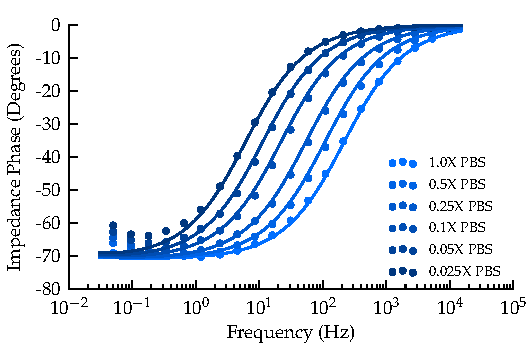
\includegraphics{graphics/displacement_impedanceVsFrequency_phase}
    \end{center}
    \caption{Phase data of interfacial impedance across electrodes 2 and 7 against frequency of a sine wave stimulus. Traces represent simulated data while markers represent measured values.}
    \label{fig:CPE_Phase}
\end{figure}

\begin{figure}
    \begin{center}
        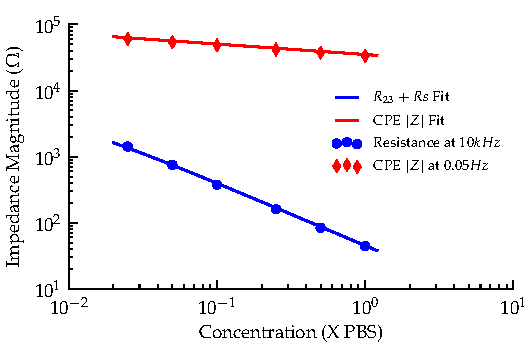
\includegraphics{graphics/scalingFactors_Displacement_IEEE}
    \end{center}
    \caption{Simulated and measured values of CPE parameters versus concentration of PBS. $|Z|$ is compared at 0.05\thinspace Hz as measured data is unaffected by $R_{S}$ at this frequency.}
    \label{fig:CPE_Scaling}
\end{figure}

\begin{table}
    \begin{center}
        \begin{tabular}{|r|l|}
            \hline
            $m$ & $1.34$ \\ \hline
            $k$ & $1.773$\\ \hline
            $|Z|\: @\: 1Hz$& $3284 \times concentration^{-0.158}$ \\ \hline
            $R_{S}$ & $13.38 \times concentration^{-0.8397} $\\ \hline
        \end{tabular}
    \end{center}
    \caption{Displacement parameter scaling}
    \label{tab:CPEparams}
\end{table}

\section{Faradaic Parameters}

With parameters fitted for the scaling of both the CPE and $R_{S}$ with PBS concentration, we evaluate Faradaic conduction. The interface model uses two reverse connected diodes to reproduce the exponential behaviour of Faradaic current conduction, implied by the Butler-Volmer equation. We wish to measure this conduction by separating it from the displacement behaviour of the CPE. By using a DC measurement technique, as opposed to cyclic measurements, we are able to separate the effects in time. 
Like a conventional capacitor, when the voltage across the CPE changes, it responds by absorbing or ejecting charge, causing a spike in current. The CPE will draw negligible current once it has settled and in the case of our model we assume the remaining current conduction to be the result of Faradaic processes. 
{\color{blue} In \cite{Greatbatch1969} it is shown that the stirring of an air-saturated solution of physiological saline reduces the settling time of platinum electrodes to stimulus transients; with both situations eventually settling to the same impedance.}
The equation governing current conduction in a diode where the forward voltage across the diode, $V_{D}$, is small is
\begin{equation}
    I = i_{0}  e^{V_{D} / n V_{T}}
\end{equation}
where $V_{T}$ is the thermal voltage and is approximately 25\thinspace mV at a temperature of 300\thinspace K. We wish to find how the saturation current ($i_{0}$) and the ideality factor ($n$) scale as the solution salinity is varied.

Faradaic measurements were made using an Agilent E5270B Precision Measurement Mainframe producing a stepped DC voltage stimulus across electrodes [TODO: Item 28] 2 and 6 whilst continuously measuring the output current. We commenced with 1.0X concentration of the stock solution (table~\ref{tab:PBSrecipe}). This solution was progressively diluted in factors of two between each measurement. The solution was mixed continuously using a standard laborotary grade magnetic stirrer. The solution was in equlibriumm with air prior to and during measurement and the electrodes remained submerged at all times.
A single measurement run involved stepping the voltage across electrodes 2 and 7 from 0.5\thinspace V to 1.2\thinspace V in increments of 0.05\thinspace V; this range was previously determined to capture the onset of Faradaic conduction.

In \cite{Cogan2008} it has been noted that results obtained using cyclic voltammetry are dependant on, among other factors, the measurement sweep rate. This indicates a lack of isolation between displacement and Faradaic mechanisms. Our measurements were repeated using wait-times of 4, 16, 32 and 64 seconds between voltage increments, allowing us to determine the effect of sweep rate. From these measurements and those of a separate investigation\footnote{We took measurements of the interface's response to voltage steps when left to settle for 10 000 seconds, of which the first 250\thinspace seconds are shown in figure~\ref{fig:CPE_currentVsTime}. Those measurements show a trend of decreasing current stabalisation time as the overpotential steps increase. Sixty four seconds after stepping from 0.64\thinspace V to 0.72\thinspace V, the current has stabalised to $95\%$ of its value at 10\,000 seconds. At overpotential steps for higher voltages, the settling time is further reduced. These measurements were made in still solution and we expect stirring will further reduce settling time.} we concluded that a wait-time of 64 seconds was sufficient.
\begin{figure}
    \begin{center}
        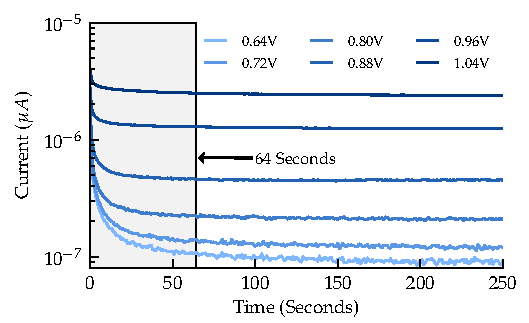
\includegraphics{graphics/CPE_currentVsTime}
    \end{center}
    \caption{Current versus time after a stepped voltage increment across a pair of interfaces. Time before 64 seconds is highlighted in grey. Measurements were taken with a wait time of 10,000 seconds between increments.}
    \label{fig:CPE_currentVsTime}
\end{figure}

In figure~\ref{fig:StepResponse_Faradaic}, electrical current measurements are plotted against time (solid lines). Each spike marks the point at which the voltage is incremented. We expect the peak current to be much higher than is shown since each measurement point is the average of 300 samples taken over 1 second. Note that the amount of charge absorbed by the CPE increases with concentration of PBS, but the current for each concentration converges to approximately the same value. Dotted lines have been added that link the electrical current measurements taken 10 seconds after each increment for 0.125X PBS (lower trace) and 1.0X PBS (upper trace). These dotted traces show results typical of cyclic methods, where the electrode overpotential is never constant. This illustrates the benefit of using DC measurements when measuring Faradaic currents.

Figure~\ref{fig:faradaic_logCurrentVsVoltage} shows the settled currents plotted on a log scale, versus the voltage applied across the electrodes. This uses the same data as the previous figure but has been processed so that each point represents the average of the final 24 current measurements at each step. Below 0.9\thinspace V it appears that the concentration of the solution had no identifiable effect on Faradaic conduction as the traces are not monotonic with concentration in this region.  Between 0.9\thinspace V and 1.05\thinspace V (concentration dependent) a transition occurs which results in current conduction becoming dependent on solution concentration.
Above 1.05\thinspace V the traces diverge showing clear dependence upon concentration.

\begin{figure}
    \begin{center}
        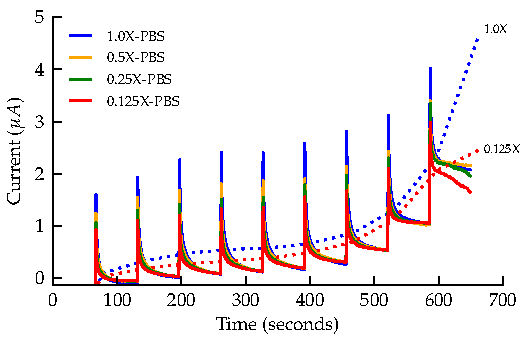
\includegraphics{graphics/currentTimeFaradaicCPE_Stacked_IEEE}
    \end{center}
    \caption{Current conduction with 0.05\thinspace V stepped voltage increments from 0.5\thinspace V to 0.9V. Each voltage is held for 64 seconds before being further incremented. Dotted lines connect current measurements occurring 10 seconds after an increment.}
    \label{fig:StepResponse_Faradaic}
\end{figure}

We attribute the change in behaviour between 0.9\thinspace V and 1.05\thinspace V to a transition to diffusion-controlled conduction.
We hypothesise that the charging of the CPE draws available ions to the electrode, creating a layer of high ionic concentration at the surface irrespective of that of the solution bulk. It is this layer that is subsequently consumed by the Faradaic reactions at a rate dependent on the log of the electrode overpotential.  The effect of bulk solution concentration while this layer has formed is negligible until the point at which the layer is consumed faster than it can be replenished. At this stage, and with increasing overpotential, the Faradaic conduction is governed by diffusion of ions from the bulk into the layer, the rate of which increases with the ion concentration in the bulk. We believe this explains the divergence of conduction with concentration between 0.9\thinspace V and 1.05\thinspace V and why there is no observable dependence on bulk ion concentration beforehand.

This hypothesis intimately links the Faradaic component to the CPE, where the latter is a precursor to the former. For the purposes of our model, we are content with placing a limit of 0.9\thinspace V across the pair of interfaces and using the assumption that Faradaic conduction does not change with concentration. Further investigation into modelling this relationship is needed in order to extend the model into the diffusion controlled scenario. We hope to publish this in a follow-up paper.

\begin{figure}
    \begin{center}
        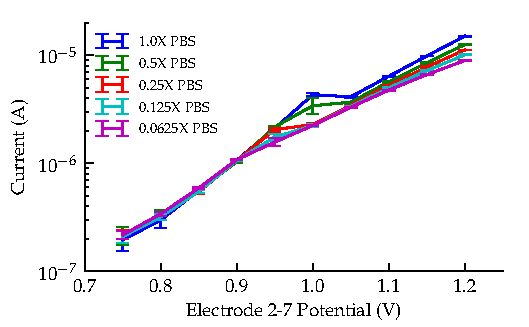
\includegraphics{graphics/currentVoltage_logY_IEEE}
    \end{center}
    \caption{Faradaic conduction as a function of voltage applied across electrodes 2 and 7. Samples shown were taken between 40 and 64 seconds after each voltage increment. Error bars indicate spread in measurement results, where 95\% of samples lie within the bars.}
    \label{fig:faradaic_logCurrentVsVoltage}
\end{figure}

\begin{figure}
    \begin{center}
        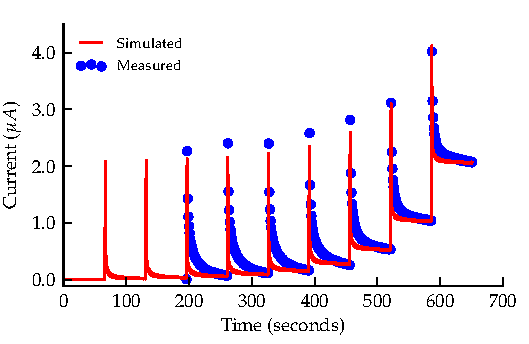
\includegraphics{graphics/faradaic_currentVsTimeIEEE}
    \end{center}
    \caption{Current versus time for 1.0X PBS overlaid with simulated results of the interface model's response to increasing voltage steps. The model used for simulation includes the CPE, diodes and $R_{S}$.}
    \label{fig:faradaic_currentVsTime}
\end{figure}

\begin{figure}
    \begin{center}
        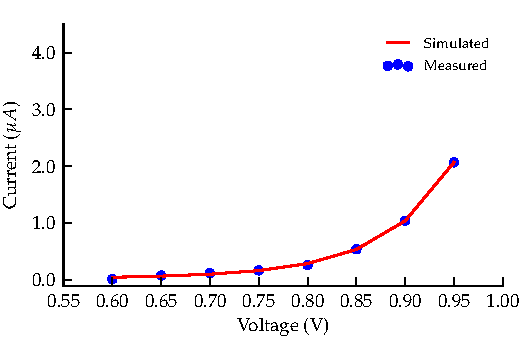
\includegraphics{graphics/faradaic_currentVsVoltageIEEE}
    \end{center}
    \caption{Simulated response of the interface model compared to measurement from the electrodes with a stepped voltage overpotential. Measurement points show current values taken at the $64^{th}$ second after each voltage increment.}
    \label{fig:faradaic_currentVsVoltage}
\end{figure}

\begin{table}
    \begin{center}
        \begin{tabular}{|r|l|}
            \hline
            $i0$ & 2.757e-12\\ \hline
            $n$ & 1.36\\ \hline
        \end{tabular}
    \end{center}
    \caption{Faradaic parameters}
    \label{tab:FaradaicParams}
\end{table}

Parameter values for $i_{0}$ and $n$ are presented in table~\ref{tab:FaradaicParams}. These parameters were found by fitting the diode equation to the results shown in figure~\ref{fig:faradaic_currentVsVoltage}.

\section{In-vivo measurements of sheep}

\begin{figure}
    \begin{center}
        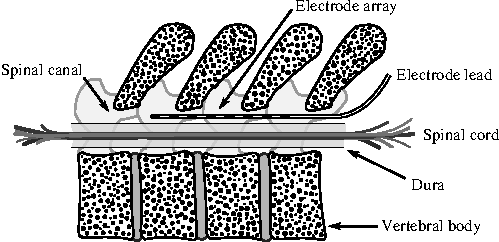
\includegraphics{graphics/sheepSpine}
    \end{center}
    \caption{Cross section of a sheep spine showing the position of the electrode array relative to the dura. Spotted regions represent cross sectioned vertebrae.}
    \label{fig:sheepSpine}
\end{figure}

We now test the claim that 0.1X PBS is a reasonable representation of the spine of a living sheep.
The displacement measurements were repeated inside the spinal canal of a live sheep, just outside the dura as shown in figure~\ref{fig:sheepSpine}. The sheep were prepared and anaesthetised using the procedures described in \cite{Parker2013} under the Animal Care and Ethics Committee approval of the Royal North Shore Hospital. The study complied with the Australian Code of Practice for the Care and Use of Animals for Scientific Purposes. The measurements are presented in figures~\ref{fig:displacement_sheepCPEMagnitude} and~\ref{fig:displacement_sheepCPEPhase} on top of the array of traces for saline taken from figures~\ref{fig:CPE_Magnitude}
and~\ref{fig:CPE_Phase}.
Although it is clear that there are complications in vivo, a 0.25X PBS saline offers a good approximation to the resistive part of the trace.
The reactive part would be better modelled by a solution of less than 0.025X concentration.


\begin{figure}
    \begin{center}
        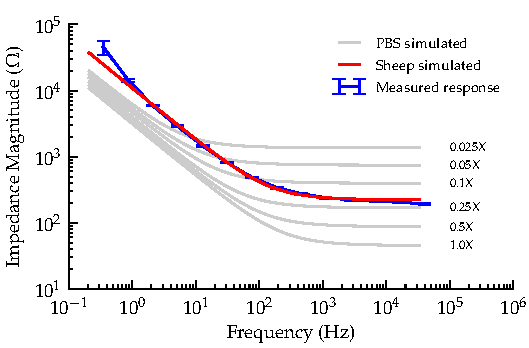
\includegraphics{graphics/displacement-withSheep_impedanceVsFrequency_magnitude}
    \end{center}
    \caption{Comparison between the magnitude of CPE in live sheep (blue circles) against each of the PBS traces from figure~\ref{fig:CPE_Magnitude} (grey lines) and a simulated fit to the sheep data (red trace).}
    \label{fig:displacement_sheepCPEMagnitude}
\end{figure}

\begin{figure}
    \begin{center}
        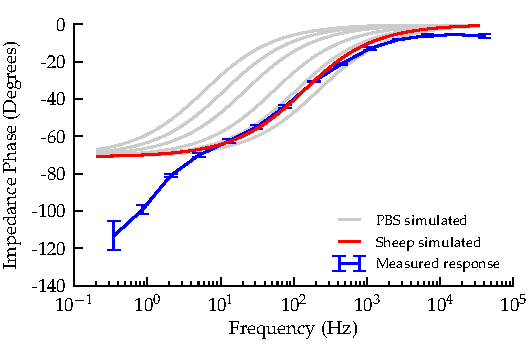
\includegraphics{graphics/displacement-withSheep_impedanceVsFrequency_phase}
    \end{center}
    \caption{Comparison between the phase response of the CPE in live sheep (blues circles) against each of the PBS traces taken from figure~\ref{fig:CPE_Phase} (grey lines) and a simulated fit to the sheep data (red trace).}
    \label{fig:displacement_sheepCPEPhase}
\end{figure}

\section{Conclusion}

We have used the parameters of a compact electrical model of an implantable electrode as a way of objectively comparing scenarios.
We have measured how changing the concentration of PBS affects the parameters of this model.
We have drawn direct relationships with concentration sufficient to predict interface characteristics at arbitrary dilutions of PBS.
We found that the magnitude of the CPE element moves much more slowly with concentration whereas the resistance moved almost linearly.
Using DC measurements we conclude that the salinity of the bulk does not affect Faradaic conduction until a threshold voltage is reached. We hypothesise that this is because the double-layer sets the effective concentration of ions in a localised volume surrounding each electrode. In-vivo measurements of platinum electrodes in sheep spine showed that no single concentration of PBS matches both the CPE and the resistive characteristics at once. Nevertheless, 0.1X PBS is a good compromise.

\section*{Acknowledgment}
The authors wish to acknowledge the The University of Waikato for financial support and Saluda Medical for the use of facilities and equipment.

\begin{thebibliography}{99}

    \bibitem{Mohtashami2011}
    Saba~Mohtashami,
    ``ELECTROCHEMICAL PROPERTIES OF FLEXIBLE ELECTRODES FOR IMPLANTED NEUROMUSCULAR EXCITATION APPLICATIONS'',
    Open Acess Dissertations and Theses (2011), Paper 6152

    \bibitem{Horch2004}
    K.~W.~Horsch and G.~S.~Gurpreet,
    ``Neuroprosthetics: theory and practice'',
    World Scientific, 2004.

    \bibitem{Cogan2008}
    Stuart~F.~Cogan,
    ``Neural Stimulation and Recording Electrodes'',
    Annu. Rev. Biomed. Eng. 2008. pp275--309.

    \bibitem{Troy2006}
    John~B.~Troy, Donald~R.~Cantrell, Allen~Taflove and Rodney~S.~Ruoff
    ``Modeling the electrode-electrolyte interface for recording and stimulating electrodes'',
    {\em Proceedings of the 28th IEEE EMBS Annual International Conference}
    New York City, USA, Aug. 30, 2006, pp879--881.

\bibitem{Franks2005}
W.~Franks, Iwan~Schenker, Patrik~Schmutz, and Andreas Hierlemann,
``Impedance Characterization and Modeling of Electrodes for Biomedical Applications'',
\emph{IEEE Transactions on Biomedical Engineering},
vol.~52 no.~7, July 2005, pp1295--1302.

\bibitem{ScottSingle2013}
Jonathan Scott and Peter Single,
``Compact Nonlinear Model of an Implantable Electrode Array for Spinal Cord Stimulation (SCS)'',
to be published in
{\em IEEE Transactions on Biomedical Circuits and Systems},
DOI: 10.1109/TBCAS.2013.2270179, 2013.

\bibitem{Kane13}
Sheryl~R.~Kane, Stuart~F.~Cogan, Julia~Ehrlich, Timothy~D.~Plante, Douglas~B.~McCreery and Philip~R.~Troyk,
``Electrical Performance of Penetrating Microelectrodes Chronically Implanted in Cat Cortex``,
{\em IEEE Transactions on Biomedical Engineering},
vol.~60 no.~8, August 2013, pp2153--2160.

\bibitem{Merrill05}
Daniel~R.~Merrill, Maron Bikson and John~G.~R.\ Jefferys,
``Electrical stimulation of excitable tissue: design of efficacious and safe protocols'',
Journal of Neuroscience Methods 141 (2005), pp171--198.

\bibitem{StJudeOctrode}
St.~Jude Medical, Octrode Percutaneous Lead for Neuromodulation,
\url{http://www.sjmneuropro.com/Products/US/Percutaneous-Leads.aspx},
retrieved December 2012.

\bibitem{Greatbatch1969}
W.~Greatbatch, B.~Piersma, F.~D.~Shannon, and S.W.~Calhoon, S. W.
``Polarization phenomena relating to physiological electrodes'',
Annals of the New York Academy of Sciences,
167(2), 1969 pp722-744.

\bibitem{Morrison59}
Ralph Morrison,
``RC Constant-Argument Driving-Point Admittances'',
{\em IRE Transactions on Circuit Theory},
September 1959, pp310--317.

\bibitem{Elwakil10}
Ahmed~S.~Elwakil,
``Franctional-Order Circuits and Systems: An Emerging Interdisciplinary Research Area''
IEEE Circuits and Systems Magazine, Fourth quarter, 2010, pp40--50.

\bibitem{Parker2013}
Parker J.L., Karantonis D.M., Single P.S., Obradovic M., Laird J., Gorman R.B., Ladd L.A., Cousins M.J.,
``Electrically Evoked Compound Action Potentials Recorded From the Sheep Spinal Cord'',
Neuromodulation 2013; 16: 295--303.

%%%%%%%%%%%%%%%%%%%%%%%%%%%%%%%%%%%%%%%%%%%%
% Check that these are in the right order!!!
%%%%%%%%%%%%%%%%%%%%%%%%%%%%%%%%%%%%%%%%%%%%

\bibitem{Weiland2000}
Weiland~James~D. and Anderson~David~J.,
``Chronic Neural Stimulation with Thin-Film, Iridium Oxide Electrodes'',
{\em IEEE Transactions on Biomedical Circuits and Systems},
vol.~47 no.~7, July 2000, pp911--918




\end{thebibliography}


\begin{IEEEbiography}[{
\includegraphics[width=1in,height=1.25in,clip,keepaspectratio]{graphics/JBSatNICTA.jpg}}]{Jonathan Scott}
(M'80--SM'99) is the Foundation Professor in
Electronic Engineering at the University of Waikato in Hamilton, New
Zealand.  From 1998 to 2006 he was with the Hewlett-Packard,
now Agilent Technologies, Microwave Technology Center in Santa Rosa,
where he was responsible for advanced measurement systems.  In 1997 and
1998 he was Chief Engineer at RF Technology in Sydney.  He was with The
University of Sydney in the Department of Electrical Engineering prior
to 1997.  He is a Professorial Fellow of Macquarie
University.  Professor Scott has authored over 100 refereed
publications and holds a number of patents.
\end{IEEEbiography}


\begin{IEEEbiography}[{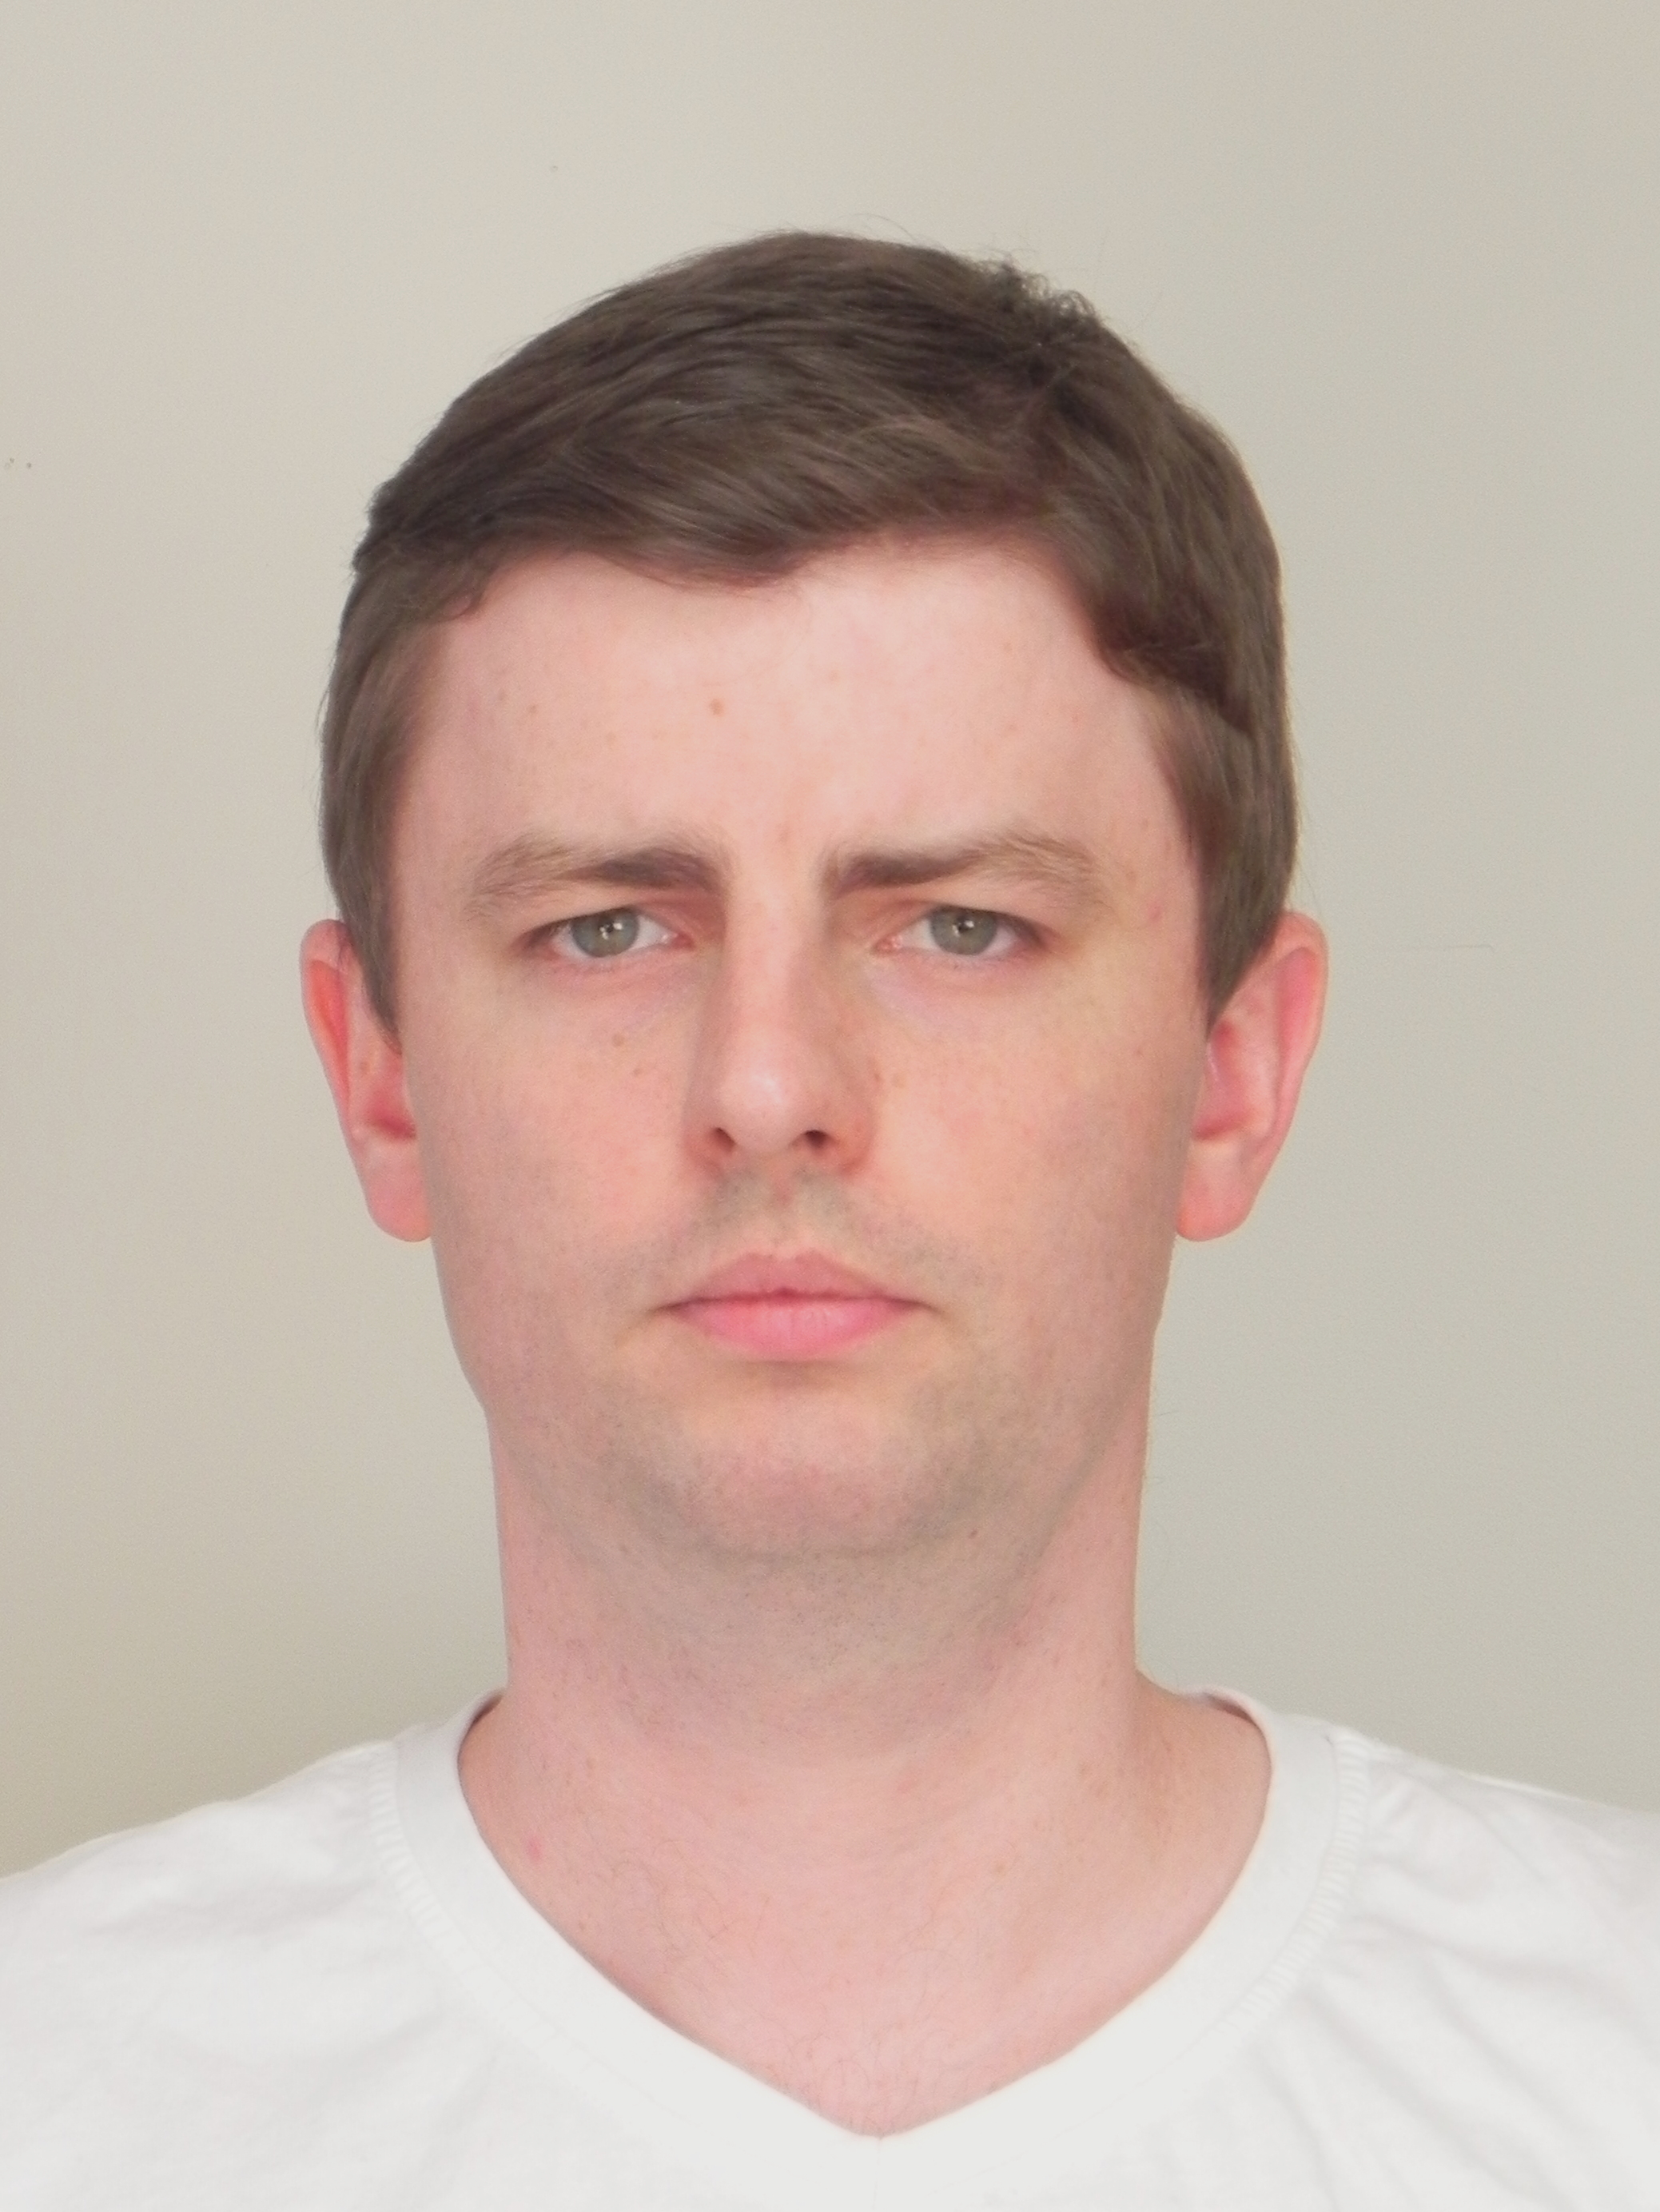
\includegraphics[width=1in,height=1.25in,clip,keepaspectratio]{graphics/MarkJones-Aug13.jpg}}]{Mark Jones}
received the B.Sc. degree in Physics in 2008 and the M.E. degree in Microwave Electronics in 2009 from The University of Waikato, Hamilton, New Zealand.
He is working towards a Ph.D. in Electrical Engineering, also at The University of Waikato.
\end{IEEEbiography}

\section*{Reviewer Comments}

\subsection*{Reviewer 1}

{\color{blue}
I am not very enthusiastic about his paper as it does not contain many novel or original ideas and finding. On the electrochemistry side it is superficial and falls back behind published state of the art and textbook knowledge.\\
{\color{OliveGreen}
    Item 1\\
    {\color{Red} Research textbook knowledge and published state of the art relating to electro chemistry in our area.}
    This response has concerned us and we have subsequently invested considerable effort in broadening our search of published state-of-the-art. Where possible we have included references to electrochemistry literature from any areas we are dealing with in this revision. During this expansion we were unable to find anything that subtracts from the novelty of this work. That said, our work is concerned primarily with the electrical side of an interface impedance and more specifically with that of an implanted electrode. Our intention is to be able to encapsulate the electrical aspect of the interface and surrounding electrolyte in a purely mathematical construct, regardless of the chemistry at play.
}\\

1. The interface model as such is not new and has been published extensively.\\
{\color{OliveGreen}
    Item 2\\
    {\color{Red} Review and discuss existing interface models}
    No response yet.
}\\

2. The authors do not at all comment on interface polarization, which is particularly important under DC conditions. As soon as an electrode carries current, such phenomena become important and relevant.\\
{\color{OliveGreen}
    Item 3\\
    {\color{Red} Is polarisation a separate mechanism from double layer formation? If so, can we address? Polarisation will be just as important in cyclic measurement techniques where the cycle time is low. Does anyone understand polarisation sufficiently to remove it from measurements? Is polarisation not just remaining charge in a layer around an electrode, is it not just the double layer?}
    No response yet.
}\\

3. To assess the resistivity or impedance of a material between two electrodes, one normally uses a 4-electrode setup with injection of current through the two outer electrodes, while measuring a voltage between the inner ones. This is particularly relevant for the measurements in Fig. 3 and the related and subsequent text.\\
{\color{OliveGreen} 
    Item 4\\
    {\color{Red} I don't understand what use doing this would be. All voltage dropped between two end electrodes, voltage proportional to total impedance between electrodes. The most use you could get from this would be to find how much is dropped across a single interface, which is exactly what we are doing.}
    No response yet.    
}\\

4. The authors never mention the origin of any Faradaic contribution at the electrodes. What is the electro- or redox-chemistry that the authors assume to happen?? Gas formation at the electrodes, electrolysis of the saline, i.e., hydrogen and oxygen formation??\\
{\color{OliveGreen}
    Item 5\\
    {\color{Red} Do we wish to get into this? Perhaps we could touch on it (after reviewing electrochemistry literature) but leave it loose and mention that it is not our intention to completely understand the mechanisims at the chemical level, rather to compare an available model with measurements and comment.}
    No response yet.
}\\

5. Figure 5 is not referenced anywhere in the text. Also the blue variations in the curves are hardly visible.\\
{\color{OliveGreen} 
    Item 6\\
    {\color{Red} Enhance color variation in Figures 4 and 5 and make a reference to Figure 5}
    Graphs redrawn with a wider range of shading to help identify traces.
}\\

6. Since the electrode model includes two back-to-back diodes, I think it would be valuable to sweep the voltage from -1.2V to +1.2V.\\
{\color{OliveGreen}
    Item 7\\
    {\color{Red} The diodes are identical, this is moving into polarisation territory again. In effect, they are both being used (one by + and other by -). I don't know what to say about this. We wanted to make all the measurements happen in as little time as possible. We have data from sweeps in the other direction, not DC though.}
    No response yet.
}\\

7. There is a big difference between blue dots and red curve in Fig. 10, except for the "voltage increment time" and "64 seconds after increment".  This indicates to me that the CPE model is NOT that accurate, as the settling curve is highly correlated to the CPE parameters.\\
{\color{OliveGreen}
    Item 8\\
    {\color{Red} This is true, try and pinpoint exactly why this is happening. Why does the CPE perform so well in the CPE frequency response plots yet so poorly in the Faradaic part?}
    No response yet.
}\\
}

\subsection*{Reviewer 2}

{\color{blue}
In this manuscript, the authors report how the non-linear electrode-electrolyte interface model parameters change as a function of saline solution concentration. This is a very interesting and important subject that could be potentially of great importance for readers of IEEE Transactions on Biomedical Circuits ans Systems. The manuscript is well written and adequately referenced. However, the reviewer would like to pose a few questions to the authors to clarify some  issues in the manuscript, which should be addressed.\\

page 2, in text/ table II. The scaling parameters and their meanings should be described more comprehensively. They remain somewhat unclear and meaningless to reader.\\
{\color{OliveGreen}
    Item 9\\
    {\color{Red} Pull in more explination from JonathanScott2013 relating to the resistor mesh}
    No response yet.
}\\

page 2 Measurement of the CPE. What was the current density used in EIS measurements?
What is the effect of chosen current density on CPE impedance (Fig. 5)?
{\color{OliveGreen}
    Item 10\\
    {\color{Red} Estimate current density and investigate possible effects}
    Maximum and minimum current density during displacement current measurement added. No comment on effect formed yet. No response yet.
}

In addition,  measurement apparatus information is fully lacking.\\
{\color{OliveGreen}
    Item 11\\
    {\color{Red} Describe instruments used in measurements or make reference to Jonathans paper}
    Added details of the instruments used to conduct inter-electrode resistance measurements and clarified thier reuse for displacement measurements.
}\\

page 2, line 52. "the magnitude shifts relatively little". However, In Fig. 4, logaritmic scale is used, and the change from 1.0X to 0.025X is almost 50k at the lowest frequencies. 
please clarify this point.\\
{\color{OliveGreen}
    Item 12\\
    {\color{Red} ``shifts relatively little'' meaning at this impedance 50k is small compared to total resistance''}
    No response yet.
}\\

page 3, in text/ table III. The parameters (m, k..) and their meanings should be described more comprehensively, as well.\\
{\color{OliveGreen} 
    Item 13\\
    {\color{Red} Describe the parameters m and k in the resistor network (pull from Jonathans paper and sub-references)}
    No response yet.
}\\

Figure 9 (page 4). There is a clear difference in behavior of faradic conduction between 0.25X (red curve) and 0.5X (green curve). Transient current occur at 0.95V (<0.25X PBS) changing to occur at 1.0 V (>0.5X PBS). This behavior has not discussed in manuscript at all. Please revise it.\\
{\color{OliveGreen}
    Item 14\\
    {\color{Red} Should be easy to do, perhaps I make a second graph that shows more of the time data}
    No response yet.
}\\

page 4. Referencing (in the text) to the Fig. 10 is lacking (?).\\
{\color{OliveGreen}
    Item 15\\
    {\color{Red} Include a reference to Figure 10 in the document}
    No response yet.
}\\

Finally, and most importantly, the part of in vivo measurements are very limited since only one spinal channel measurement has been performed. My opinion is that this manuscript could be even better without this uncertain (n=1) result and thus I recommend to leave this part out.\\
{\color{OliveGreen}
    Item 16\\ 
    {\color{Red} Leave sheep in but perhaps show the second measurement (day 1) if possible (4th reviewer found sheep correlation to PBS result interesting). Would a separate sheep measurement graph be of use showing all sheep results? Or do we hold onto this for the better phantom paper?}
    No response yet.
}\\
}

\subsection*{Reviewer 3}

{\color{blue}
Authors
The aim of this paper, to find a SPICE model of implanted electrodes, is important and the results presented in the paper are interesting. However, as it stands the paper is not well written and must be revised. The weaknesses of the paper are an unclear structure, with results and discussion mixed, poor attention to detail and inaccurate use of words.\\
{\color{OliveGreen}
    Item 17\\
    {\color{Red} Revise poor use of words (perhaps relating to model elements/physical elements). Perhaps separate the results and discussion sections.} 
    No response yet.
}\\

Concerning the experiments, I have two points to make.

1. You do not explain how the impedance measurements have been made (Figs 4, 5 13 & 14). I want to know how much charge was being applied to these electrodes at low frequencies (e.g. 0.05 Hz): what potential excursion occurred was it really a ``small signal''?\\
{\color{OliveGreen}
    Item 18\\
    {\color{Red} Estimate the amount of charge being injected in each of the measurements (fits with the current density)}
    Instrumentation for CPE measurements have been added. I have also added current density and peak stimulus voltage information to displacement current measurement. [TODO: Calculate and add total charge transfer for both CPE and Faradaic].
}\\

2. I think that the classical view of the electrochemistry of Pt in saline (as, for example, expressed in your ref 1), is that the electrolysis reactions (oxygen and hydrogen evolution) start with a potential difference of about 1.4V. Below this p.d., the likeliest reaction is reduction of oxygen at the cathode which could accompany oxygen evolution from water at the anode. Your paper lacks any consideration of the chemistry but this is a important fault in the stepped-current experiment. Was the solution in equilibrium with air before the experiment? If this is a model for electrodes in vivo, should not the PBS have been in equilibrium with gas with the in vivo partial pressure of oxygen? I suggest that you repeat this experiment, at least (i) under air, (ii) under nitrogen, & perhaps (iii) under in vivo partial pressure of oxygen. The stirring arrangements ought to be exactly described too because liquid flow may be critical.\\
{\color{OliveGreen}
    Item 19\\
    {\color{Red} This represents a lot of work to redo the measurements. Perhaps we make it clear that we don't know the electrochemistry side, that it's simply out of our depth, and any hypothesis we draw based on electrochemistry may harm the validity of our work. If we explain more exactly the proceedure we took so as to be more repeatable and hint that we're not interested at this point on the electrochemistry, that we only wish to make the model behave like the solution.}
    No response yet.
}

Other points

1. P1, top RH col. ``0.1X'' ought to be explained when you first use this form.\\
{\color{OliveGreen}
    Item 20\\
    {\color{Red} Replace ``A 0.1X concentration'' with ``a one-tenth concentration...'' and explain exactly what that means.}
    Yes, thank you, see amendment.
}\\

2. Should the resistor model of the volume conductor from [4] be shown in this paper? It would make the paper easier to understand for your reader if you showed the model. If you are not going to do so, you might help them by saying something like ``Readers are advised to see [4] to understand the meaning of the parameters in Table II''.\\
{\color{OliveGreen}
    Item 21\\
    {\color{Red} Leave until the end, if we have the space then we put it in, otherwise put a better reference to ScottSingle2013}
    No response yet.
}\\

3. You say (p2 line 43) that there are 2 independent scaling factors. Is Rli independent or not? If not, why input it in Table II?\\
{\color{OliveGreen}
    Item 22\\
    {\color{Red} Mention that $R_{li}$ is not independent because of the geometric simplification of the resistor network. Mention that for more detail we suggest viewers read the relevant section of ScottSingle2013}
    No response yet.
}\\

4. In the legend of Fig 4 and in paragraph below, you say this is magnitude of the CPE. But surely it is not since the sloping lines become horizontal. It is the CPE in series with something. But what is this something? Is it the total series resistance or have you already subtracted the volume resistance (found in section II)?\\
{\color{OliveGreen}
    Item 23\\
    {\color{Red} Reword the caption of Fig. 4 to include the series resistance.}
    Thank you, have reworded the caption in Figure 4 to more accuratly describe the situation.
}\\

5. The previous point is complicated by your statement that Rs (Fig 2) is an addition to the volume resistance (p2 RH col). Why is Rs necessary? Is it because the resistance values at high frequencies in Fig 4 are not consistent with the values from the resistor network found in section II? If so, this would be very interesting and I would like you to bring this out.\\
{\color{OliveGreen} 
    Item 24\\
    {\color{Red} His reasoning is correct, it is because the impedance does not match at high freq. I had the graph with dotted lines to show the difference that Rs made. Jonathan, you thought this was too messy and it was removed, should it be added back in again?}
    No response yet.
}\\

6. P2, col 2, line 24: why 2 & 7?\\
{\color{OliveGreen}
    Item 25\\
    {\color{Red} Explain more clearly why electrodes 2 and 7 were chosen (to avoid end effects)}
    No response yet.
}\\

7. P2, col 2, line 53: ``implying that its behaviour is a property of Pt and water''. Previous authors have thought this showed that the CPE depended on the geometry (surface roughness) of the electrode. Did you mean that, or were you thinking of the electrochemical properties of Pt. Please make clearer.\\
{\color{OliveGreen}
    Item 26\\
    {\color{Red} We aren't sure of either but further work into the surface area of the electrode via ottonisation should reveal whether surface area is a factor - read: followup publication}
    No response yet.
}\\

8. You do not explain why, in eq 1, you want to use this form. Why nVt? I suppose it isso you can use a standard SPICE form rather than this suits the data. Is that right?\\
{\color{OliveGreen} 
    Item 27\\
    {\color{Red} Investigate other forms, comment on why this has been chosen}
    No response yet.
}\\

9. P3, col 2, line 31: why 2 and 6?\\
{\color{OliveGreen}
    Item 28\\
    {\color{Red} Took resistance measurements of lead and electrode 2 is open circuit inside the electrode. Must have meant 3 and 7, due to damaged electrode 2}
    No response yet.
}\\

10. P3, col 2, line 36. I guess you mean what is usually called a Magnetic Stirrer. Not ``inductive'' surely?\\
{\color{OliveGreen} 
    Item 29\\
    {\color{Red} What I originally thought, I don't know where inductive stirrer came from}
    Changed mention of inductive stirrer to magnetic stirrer.
}\\

11. P3 footnote. ``The response of the CPE'': this is confusing! Surely this is the response of a pair of electrodes? The CPE is an element of your model.\\
{\color{OliveGreen} 
    Item 30\\
    {\color{Red} This must form part of the inaccurate use of words comment. It's not right to say response of a pair of electrodes since there are other effects. Reword.}
    Removed reference to the CPE element and have better quantified the settling period in that footnote.
}\\

12. Fig 11 legend ``Simulated and measured response of the interface model''. Surely you mean ``Simulated response of the interface model compared to measurement from the electrodes''?\\
{\color{OliveGreen}
    Item 31\\
    {\color{Red} Yes, this is better. Replace with this.}
    Yes, that is better - thank you.
}\\

13. P5, col 2, line 46 ``the CPE is setting''. Again, you are confusing an element of your model with reality.\\
{\color{OliveGreen}
    Item 32\\
    {\color{Red} Correct, maybe a diargam of the hypothesis is required - nobody seemed to dispute the hypothesis. Check there is no ``textbook knowledge'' explanation for this beforehand.}
    Changed references to the CPE model element in the conclusion to the electrical double layer.
}\\

14. P5, col 1, line 49 ``a 0.25X PBS is a good model''.  This seems a very feeble comment on an interesting result. The series resistance part of the in vivo magnitude is a good fit to the 0.25X curve and the slope of the CPS is very similar (though you have exaggerated this by extrapolating nearly 2 decades in frequency below the lowest-frequency measurement). But the impedance at low frequencies is about three times too high. How do you explain that? It cannot be because of the bone and other high-resistivity structures around the electrodes (which would have an effect on the high frequency asymptote). So what is it? Did you measure the electrodes again in PBS after removing from the sheep? Troyk published an interesting paper with measurement from electrodes in brain of zebra finches which showed that anomalous characteristics in vivo vanished as soon as the electrodes were returned to PBS, implying that the phenomenon was not due to some biofilm deposited on the electrodes.\\
{\color{OliveGreen}
    Item 33\\
    {\color{Red} True, a feeble comment on PBS match. It may be worth noting the phase of measured data in sheep indicating that the sheep itself was reactive. There may be data at those lower points (to justify extrapolating), check. Have we measured the electrodes again since inserting into the sheep, I think we have but check.  Read the paper by Troyk, comment on applicability. Maybe there is test data between sheep in saline showing the electrodes returning to normal, check.}.
    No response yet.
}\\
}

\subsection*{Reviewer 4}
{\color{blue}
In this manuscript, the authors studied the impedance of a commercial electrode array as a function of concentration of phosphate buffered saline (PBS), both through simulation and empirical measurements, and compared those results to the impedance measured when the electrode array was implanted into a sheep's spinal cavity. From this comparison, they concluded that the current practice of testing spinal cord stimulator in 0.1x of physiologically normal saline is adequate but suggest that no single concentration of PBS captures the frequency dependence of the in vivo measured impedance.\\

Overall, the paper was brief and to the point, which in this case is actually a determent instead of a benefit. Much of the underlying theory and development of parameters appear without informing the reader of their purpose or how they were calculated and/or measured. 
For example, the parameters in Table 2 (and reported to be in Figure 3) are not explained and what their relationship to the remainder of the manuscript is not provided. 
{\color{OliveGreen}
    Item 34\\
    {\color{Red} Explain parameters in table two better or refer readers to ScottSingle2013}
    No response yet.
}
To make this manuscript more approachable to a wider audience, I recommend the authors more fully develop Sections II, III, and IV. Further, they should explain their testing in terms of standard electrochemical characterization, detailing their counter, working, and reference electrodes used in measuring impedance. 
{\color{OliveGreen}
    Item 35\\
    {\color{Red} Try to include any relevant electrochemical information, find out what that is first}
    No response yet.
}
As part of this expansion, the references should be increased beyond the present ten references. Although their current references include clearly important electrode characterization references (Cogan, Merrill et. al, & Kane et. al), the information contained in these references are not effectively used to support the authors’ work.\\
{\color{OliveGreen}
    Item 36\\
    {\color{Red} Perhaps Troyk could be added. A search for textbook knowledge and more published state of the art should uncover more references}
    No response yet.
}\\

Technically, I found one issue with this paper. In Figure 11, the x-axis labels should have 2 digits after the decimal. As presently shown, each of the labels 0.6, 0.7, ..., 1.0 are repeated twice on the axis. Presumably, the second version of the labels should be 0.65, 0.75, ..., 1.05.\\
{\color{OliveGreen}
    Item 37\\
    {\color{Red} Definitely, how did I miss that?}
    No response yet.
}\\
}
\end{document}
